\part {Fisica 2}
\chapter{programma}
\section{Base}
\begin{itemize}
	\item \textit{Elettrostatica nel vuoto} - carica elettrica, legge di Coulomb, campo elettrico, teorema di Gauss e $1^a$ equazione di Maxwell, potenziale elettrico, dipolo elettrico, conduttori, capacità elettrica, sistemi di condensatori, collegamento in serie e in parallelo, energia del campo elettrostatico.
	\item \textit{Corrente elettrica stazionaria} - resistenza elettrica e legge di Ohm, effetto Joule, forza elettromotrice e generatori elettrici, circuiti in corrente continua.
	\item \textit{Magnetismo nel vuoto} - forza di Lorentz, vettore induzione magnetica, forze magnetica
	 su una corrente, momento magnetico della spira percorsa da corrente, relazione tra momento
	 meccanico e momento magnetico, campi generati da correnti stazionarie, legge di Biot e Savart (campo
	 del filo indefinito, della spira circolare e del solenoide), 2a equazione di Maxwell, teorema di Ampère.
	\item \textit{Campi magnetici variabili nel tempo} - induzione elettromagnetica , legge di 
	Faraday-Newmann, $3^a$ e $4^a$ equazione di Maxwell, autoinduzione, circuito RL, 
	energia magnetica.
	\item \textit{Onde} - equazione d'onda, tipi di onde, velocità di fase, equazioni delle onde
	elettromagnetiche e loro proprietà, onda piana e onde sferiche, energia di un'onda 
	elettromagnetica e vettore di Poynting, spettro della radiazione elettromagnetica. 
\end{itemize}
\section{Argomenti aggiuntivi}
\begin{itemize}
	\item \textit{Elettrostatica nella materia} - la costante dielettrica, interpretazione microscopica, suscettibilità elettrica.
	\item \textit{Magnetismo nella materia} - vettori B, H e M, materiali paramagnetici, ferromagnetici, diamagnetici, legge di Curie, ciclo di isteresi.
\end{itemize}

\chapter{La legge di Couloumb}
\section{Introduzione}
L'elettromagnetismo costituisce il fondamento su cui sono costruiti i computer,
le radio e televisori, le telecomunicazioni, illuminazioni ecc.
L'elettromagnetismo spiega come gli atomi siano tenuti insieme, come
avvengono i fulmini, le aurore e gli arcobaleni. Gli antichi filosofi greci
scoprirono che l'ambra strofinata attrae pagliuzze sottili e che pietre
magnetiche naturali attraggono pezzetti di ferro. Tra i tanti scienziati che
svilupparono l'elettromagnetismo moderno, notiamo il fisico sperimentale
\texttt{Michael Faraday} ed il teorico \texttt{James Clerk Maxwell}.
\subsection{La carica elettrica}
Una bacchetta di vetro strofinata con seta si \texttt{allontana} da un'altra
bacchetta di vetro strofinata con della seta.
\begin{enumerate}
	\item \textit{Forza repulsiva} - Una bacchetta di vetro strofinata con
		della seta si \textit{avvicina} ad una bacchetta di plastica strofinata
		con la pelle di camoscio.
	\item \textit{Forza attrattiva} - Le forze sono dovute alla \textbf{carica
		elettrica}.
\end{enumerate}
Esistono due tipi di carica:
\begin{enumerate}
	\item Carica positiva, contrassegnata con il segno +;
	\item Carica negativa, contrassegnata con il segno -
\end{enumerate}
Si definisce neutro un oggetto che ha le cariche positive e negative
perfettamente bilanciate.
Spostando la carica da un oggetto all'altro, si crea una carica in eccesso.
L'oggetto può scaricarsi con scintille oppure con l'umidità dell'aria.
\subsubsection{Le proprietà delle cariche}
\begin{enumerate}
	\item Le particelle cariche dello \textit{stesso segno} si respingono;
	\item Le particelle di carica opposta si attraggono;
	\item Se strofiniamo il vetro con un panno di seta risulta in una
		\textit{carica potenziale} nel vetro;
	\item Strofinando della plastica con della pelle di camoscio si ottiene una
		\textit{carica negativa} sulla stessa.
\end{enumerate}
\subsubsection{Conduttori e isolanti}
In natura esistono le seguenti tipologie di materiali:
\begin{tasks}{2}
	\task I conduttori - le cariche si muovono liberamente;
	\task Gli isolanti - le cariche non si muovono, per l'appunto restano
	isolate;
	\task I semiconduttori - le cariche si muovono, ma il materiale possiede un
	alta resistenza;
	\task I superconduttori - le cariche si muovono senza incontrare ostacoli
	di sorta.
\end{tasks}
\newtheorem{pcariche}{Particelle Cariche}
\begin{pcariche}
	La materia composte di atomi. Gli atomi hanno un \textbf{nucleo} con
	\begin{itemize}
		\item Protoni - cariche positive;
		\item Elettroni - carica negativa.
	\end{itemize}
	La carica dell'elettrone e del protone hanno la stessa intensità ma segno
	opposto. Gli elettroni sono \textbf{attratti verso il nucleo}. Nei
	conduttori, alcuni elettroni sono \textit{liberi di muoversi}, un isolante
	\textit{non ha elettroni liberi}.
\end{pcariche}
\subsection{Carica indotta}
Una carica negativa \textit{respinge} gli elettroni nel rame, risulta una
carica positiva indotta vicino alla carica esterna. Risulta una \textbf{forza
attrattiva} tra una carica negativa e un conduttore, Anche per una carica
positiva ed un conduttore la forza risulta \textbf{attrattiva}.
\section{Legge di Coulomb}
Tra due cariche puntiformi esiste una \textit{forza elettrostatica}. La forza è
diretta \textit{lungo la retta congiungente} le due cariche.
Se le cariche sono della stessa polarità le stesse si respingono, invece, se
sono di carica opposta, avviene un attrazione tra le cariche.
\subsubsection{Riassunto sui vettori}
\paragraph{Componenti:}
\begin{equation}
	F_x=F\cos 0;\text{ }F_y=F\sin 0
\end{equation}
\paragraph{Modulo e angolo:}
\begin{equation}
	F=\abs{\vec{F}}=\sqrt{F_x^2+F_y^2};\text{ } \tan 0 =\frac{F_y}{F_x}
\end{equation}
\paragraph{Versore:}
\begin{equation}
	\hat{a}=\frac{\vec{a}}{\abs{\vec{a}}}=\frac{\vec{a}}{a}
\end{equation}
\paragraph{Sommare:}
\begin{equation}
	\vec{F}=\vec{F}_1+\vec{F}_2\to F_x=F_{1x}+F_{2x};\text{ } F_y=F_{1y}+F_{2y}
\end{equation}
La forza di una carica $q_1$ in presenza di un'altra $q_2$ è:
\begin{equation}
	\vec{F}_{12}=k\frac{q_1q_2}{r^2}\hat{r}
\end{equation}
Dove $k=8,99*10^9Nm^2C^{-2}$ è la \textbf{costante di Coulomb} e $\vec{r}$ è il
vettore di lunghezza pare alla distanzia $q_2$ a $q_1$.
\begin{enumerate}
	\item Se $q_1$ e $q_2$ hanno la stessa polarità, il prodotto $q_1q_2$ è 
		\textbf{positivo} e la forza è \textit{repulsiva}.
	\item Se $q_1$ e $q_2$ hanno la polarità \textbf{opposta}, il
		prodotto $q_1q_2$ è \textbf{negativo} e la forza è \textit{attrattiva}.
\end{enumerate}
La forma è una coppia di azione-reazione: $\vec{F}_{21}=-\vec{F}_{12}$
\subsection{Unità do misura}
L'unità di carica nel SI è il \texttt{Coulomb} (\ref{}). La derivata del unità
fondamentale di corrente elettrica, \textbf{Ampere}. La corrente \textit{i} è
data dal rapporto $\frac{dq}{dt}$ con cui transita la carica \textit{q}: 
$i=\frac{dq}{dt}$.
Risulta $1C=1As$
\subsection{La costante dielettrica del vuoto}
La costante di \textit{Coulomb} viene anche espressa come
$k=\frac{1}{4\pi\xi_0}$ dove $\xi_0 = 8,85*10^{-12}C^2N^{-1}m^{-2}$ è la
\textbf{constante dielettrica del vuoto}.\\
Così scriviamo $\vec{F}=\frac{q_1q_2}{4\pi\xi_0r^2}\hat{r}$, o per ottenere il
modulo $F=\frac{\abs{q_1}\abs{q_2}}{4\pi\xi_0r^2}\hat{r}$
\subsection{Forze multiple}
Le forze elettrostatiche obbediscono al \textbf{principio di sovrapposizione}.
Se molte particelle sono vicine alla carica $q_1$, la forza netta è $\vec{F}_{1,net}=\vec{F}_{12}+\vec{F}_{14}+\dots+\vec{F}_{1n}$.
\paragraph{Attenzione:} \textit{somma vettoriale!}
\section{Teorema del guscio}
\begin{tasks}(2)
  \task Primo teorema del guscio:\\
  \textit{Una superficie sferica uniformemente carica attrae o respinge una carica esterna come se tutta la carico fasse concentroto
    nel suo centro}.
  \task Secondo teorema del guscio:\\
  \textit{Uno carico posto all'interno di uno superficie chiusa uniformemente carica non ne sente la foza}.
\end{tasks}
\section{La quantizzazione della carica}
Qualunque carica \textit{q} può essere scritta come $q=ne$ in cui $n=\pm 1,\pm 2, \pm 3, \dots$ ed è la carica elementare: $e = 1,602*10^{-19}C$
\begin{tasks}
  \task Il \textbf{protone} ha carica $+e$
  \task L'ettrone ha carica $-e$
\end{tasks}

Il valore di e è così piccolo che normalmente la granularità non appare nei fenomeni di larga scala. Attraverso un filo con corrente di 1A passano circa $6,2*10^{18}$ elettroni al secondo.

\section{La conservazione della carica}
La carica elettrica è conservata - Lo strofinamento del vetro con un panno di seta non crea carica positiva, ma trasferisce elettroni dal vetro alla seta. Anche nei processi nucleari la carica totale rimane invariata.
\section{Verifica}
\begin{enumerate}
\item Indicare il verso della forza che agisce sul protone centrale
\item Ordinare i tre casi secondo i valori decrescenti del modulo della forza netta sull'elettrone.
\end{enumerate}
\paragraph{Soluzione primo problema}
\begin{equation}
  q_1=+e,q_2=+2e, \text{ } R=2cm.
\end{equation}
Calcolo la forza $\vec{F}_{12}$
\begin{equation}
  F_{12}=k\frac{\abs{q_1}\abs{q_2}}{R^2}=k\frac{2e^2}{R^2}=\frac{8,99*10^9*2*(1,6*10^{19})}{R^2}=1,15*10^{-24}N
\end{equation}
Quindi il valore finale è $\vec{F}_{12}=-(1,15*10^{-24}N)\hat{x}$
\begin{equation}
  q_1=+e, q_2 = +2e,q_3=-2e, R=2cm.
\end{equation}
Calcolo la forza $\vec{F}_{1,net}$
\begin{equation}
 F_{13}=k\frac{2e^2}{\left(\frac{3}{4}R\right)^2}=2,05*10^{-24}N
\end{equation}
Quindi il valore che otteniamo è $F_{13}=(2,05*10^{-24}N)$
\begin{equation}
  \begin{matrix}
  \vec{F}_{1,net}=\vec{F}_{12}+\vec{F}_{13}=-(1,15*10^{-24}N)\hat{x}+(2,05*10^{-24}N)
    \hat{x}\\=(0,90*10^{24}N)\hat{y}=-(0,125*10^{-24}N)\hat{x}+(1,775*10^{-24}N)\hat{y}
  \end{matrix}
\end{equation}
Quindi il valore che otteniamo è $F_{1,net,x}=\sqrt{F^2_{1,net,x}+F^2_{1,net,y}}=1,78*10^{-24}N$
\paragraph{Soluzione secondo problema}
$q_1=8e,\text{ } q_2=-2e$. In che punto un protone è in equilibrio?
\begin{equation}
  \begin{matrix}
    \vec{F}_1+\vec{F}_2=0. \text{ } x>L.\text{ } \frac{kq_1e}{x^2}+\frac{kq_2e}{(x-L)^2}=0\\
    \to \left(\frac{x-L}{x}\right)=\frac{-q_2}{q_1}=\frac{1}{4}\to \frac{x-L}{x}=\frac{1}{2}\to x=2L
  \end{matrix}
\end{equation}


\chapter{Campi elettrici}
\section {L'aspetto fisico}
La forza elettrostatica tra 2 cariche sembra una ``azione a distanza''
\begin{itemize}
\item Spiegazione alternativa:\\
  \textit{La carica 1 crea un campo elettrico nello spazio circostante}\\
  \textit{La carica 2 sente l'effetto del campo 1}\\
\item vice versa:\\
  \textit{La carica 2 crea un campo elettrico nello spazio circostante}\\
  \textit{La carica 1 sente l'effetti del campo 2}
\end{itemize}
\section {Il campo elettrico}
\begin{tasks}{2}
\task campo scalare: temperatura, pressione, densità
\task campo vetoriale: velocità, accelerazione, forza
\end{tasks}
La forza $\vec{F}$ su un \textbf{carica esplorativa} $q_0$ determina il campo elettrico $\vec{E}$:
\begin{equation}
  \vec{E}=\frac{\vec{F}}{q_0}
\end{equation}
$\vec{E}$ è un campo vettoriale. Nel SI ``Sistema Internazione'', si esprime in N/C (o V/m)
\section{Linee di campo elettrico}
Per visualizzare $\vec{E}$, disegnamo delle linee:
\begin{itemize}
	\item Il vettore $\vec{E}$ è \textbf{tangente} alla linea 
	\item La \textbf{densità} delle linee rappresenta $\abs{\vec{E}}$
        \item Le linee \textbf{escono} dalle cariche positive
        \item Le linee \textbf{entrano} nelle cariche negative
\end {itemize}
\section {Altro esempio delle linee di campo}
\begin{figure}[!h]
 	\centering
	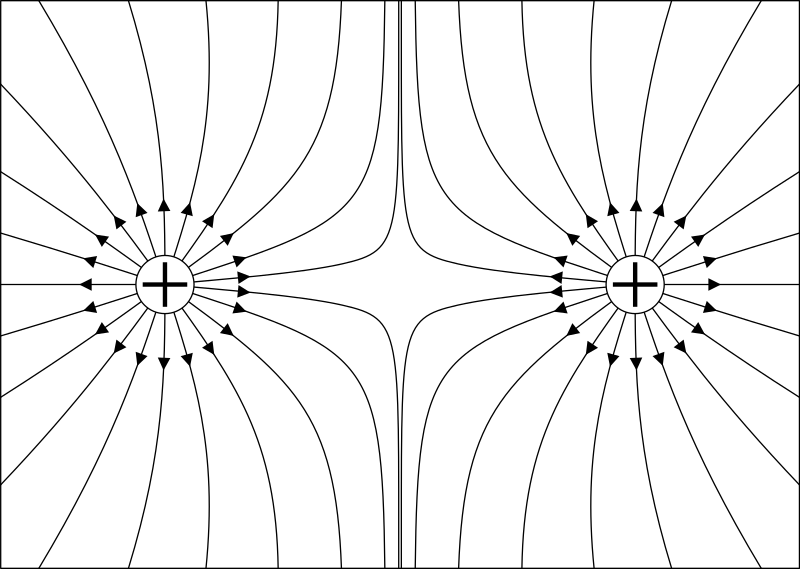
\includegraphics[height=4cm]{img/linee elettriche repulsione.png}
\end{figure}
Due cariche positive identifiche\\
Sempre:
\begin{itemize}
\item Il vettore $\vec{E}$ è tangente alla linea
\item La densità delle linee rappresenta $\abs {\vec{E}}$
\item Le linee escono dalla cariche positive
\item Le linee entrano nelle cariche negative
\end{itemize}
Il disegno stesso suggersce l'idea di una repulsione
\section{Campo $\vec{E}$ di una carica puntiforme}
Una carica esploratrice positiva $q_0$ attorno ad una \textit{carica puntiforme} $q$ sente una forza $\vec{F}=\frac{qq_0}{4\pi \xi_0r^2}\hat{r}$. \\
Per il campo $\vec{E}$ troviamo:
\begin{equation}
	\vec{E}=\frac{\vec{F}}{q_0}=\frac{q}{4\pi \xi_0r^2}\hat{r}
\end{equation}
La direzione di $\vec{E}$ è \textbf{radiale}
\begin{enumerate}
\item Per $q>0$, il verso di $\vec{E}$ è uscente
\item Per $q<0$, il verso di $\vec{E}$ è entrante
\end{enumerate}
Per il \textbf{modulo:} $E=\abs{\vec{E}}=\frac{\abs q}{4\pi \xi_0r^2}$  
\section{Il principio di sovrapposizione}
In presenza di \textbf{più cariche}, le forze obbediscono al principio di sovrapposizione:
\begin{equation}
  \vec{F}_0=\vec{F}_{01}+\vec{F}_{02}+\dots+\vec{F}_{0n}
\end{equation}
Il principio di sovrapposizione vale anche per $\vec{E}$:
\begin{equation}
  \vec{E}=\frac{\vec{F}_0}{q_0}+\frac{\vec{F}_{01}}{q_0}+\frac{\vec{F}_{02}}{q_0}+\dots+\frac{\vec{F}_{0n}}{q_0}=\vec{E}_1+\vec{E}_2+\dots+\vec{E}_n
\end{equation}
Il campo $\vec{E}$ di più particelle cariche è la somma vettoriale dei singoli contributi
\section{Verifica}
\begin{center}
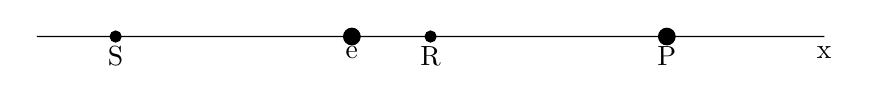
\begin{tikzpicture} 
 \filldraw 
(0,0) circle (0pt) node[align=left,   below] {}      --
(1,0) circle (2pt) node[align=center, below] {S}     -- 
(4,0) circle (3pt) node[align=right, below] {e}     -- 
(5,0) circle (2pt) node[align=right,  below] {R}     --
(8,0) circle (3pt) node[align=right, below] {P}     --
(10,0) circle (0pt) node[align=left, below] {x};
\end{tikzpicture}
\end{center}
Il disegno mostra un elettrone ($e$) e un protone ($p$) sull'asse $x$
\begin{itemize}
	\item Indicare la direzione di \textit{E} dovuta all’elettrone nel
           punto \textit{S} e nel punto \textit{R}
        \item Indicare la direzione di \textit{E} dovuta al protone nel
punto \textit{S} e nel punto \textit{R}
\end{itemize}
\subsection {Soluzione}
\begin{equation}
  \begin{matrix}
    q_1=+2e\\
    q_2=-2e\\
    q_3=-4e
  \end{matrix}
\end{equation}
Ovviamente il primo passo da fare è quello di ricavare $\vec{E}$ nel origine
\begin{equation}
  E_1=E_2=\frac{2e}{4\pi\xi_0d^2}
\end{equation}
\begin{equation}
	E_3=\frac{4e}{4\pi\xi_0d^2}
\end{equation}
Ora ricaviamo $E_x$ tramite una somma tra $E_{1x}$, $E_{2x}$ e $E_{3x}$.
\begin{equation}
	E_x=E_{1x}+E_{2x}+E_{3x}=\frac{2e}{4\pi\xi_0d^2}\cos{30^o}+\frac{2e}{4\pi\xi_0d^2}\cos{30^o}+\frac{4e}{4\pi\xi_0d^2}\cos{30^o}=\frac{8e}{4\pi\xi_0d^2}\cos{30^o}
\end{equation}
\begin{equation}
	E_x=E_{1y}+E_{2y}+E_{3y}=\frac{-2e}{4\pi\xi_0d^2}\cos{30^o}+\frac{-2e}{4\pi\xi_0d^2}\cos{30^o}+\frac{4e}{4\pi\xi_0d^2}\cos{30^o}=0
\end{equation}
\section{Campo $\vec{E}$ di un dipolo elettrico}
Due particelle cariche, $-q$ e $+q$ separate da distanza $d$ e sull'asse dipolare $z$. Il prodotto $qd$ viene chiamato \textbf{momento di dipolo elettrico}: $p=qd$ e $\vec{p}$ vettoriale.
\begin{itemize}
\item direzione: l'asse dipolare
\item verso: da $-q$ a $+q$
\end{itemize}
Il campo $\vec{E}$ sull'asse dipolare distante $z$ dal centro del dipolo:
\begin{equation}
  \begin{matrix}
    E=E_+-E_-=\frac{q}{4\pi \xi\left(z-\frac{d}{2}\right)^2}-\frac{q}{4\pi \xi\left(z-\frac{d}{2}\right)^2}
    =\frac{q}{4\pi\xi_0}\frac{\left(z-\frac{d}{2}\right)^2-\left(z-\frac{d}{2}\right)^2}{\left(z-\frac{d}{2}\right)^2\left(z-\frac{d}{2}\right)^2}
    =\frac{q}{4\pi\xi_0}\frac{2zd}{\left(\left(z-\frac{d}{2}\right)^2\right)^{2}}\\
    =\frac{qd}{2\pi\xi_0z^3}\left(1-\left(\frac{d}{2z}\right)^2\right)^{-2}
    \end{matrix}
\end{equation}
Per $z>>d$ troviamo $E(z)=\frac{p}{2\pi\xi_0z^3}$, anche fuori dell'asse $z$, $E\propto r^{-3}$ per $r>>d$\\
Materiale isolandte (\textbf{e. g. plastica}). Raggio \textit{R}, carica \textbf{superficiale} $\sigma$ - Punto \textit{P} sull'asse centrale, direzione \textit{z}. Ogni anello ha carica $dq=\sigma 2\pi rdr$ e contribuisce a $dE=\frac{zdq}{4\pi\xi_0\left(4r^2+z^2\right)^{\frac{3}{2}}}$
\begin{equation}
  E=\inf dE=\int^R_0\frac{z\sigma2\pi rdr}{4\pi\xi_0\left(4r^2+z^2\right)^{\frac{3}{2}}}=\frac{z\sigma}{4\xi_0}\left[\frac{\left(4r^2+z^2\right)^{-\frac{1}{2}}}{-\frac{1}{2}}\right]^R_0
\end{equation}
Il risultato è $E=\frac{\sigma}{2\xi_0}\left(1-\frac{z}{\sqrt{R^2+z^2}}\right)$. Per $z<<R$ troviamo $E=\frac{\sigma}{2\xi_0}$.\\
Su una carica $q$ in un campo elettrico esterno $\vec{E}$ agisce un forza elettrostatica $\vec{F}=q\vec{E}$
\begin{itemize}
  \item per $q>0$, $\vec F$ ha lo stesso orientamento di $\vec E$
  \item per $q<0$, $\vec F$ ha l'orientamento opposto di $\vec E$
\end{itemize}
NB: Una carica non sente il proprio campo elettrico esterno!
\section{Misura della carica elementare}
\subsection{Millikan 1910}
\fbox{
 	\addtolength{\linewidth}{-2\fboxsep}%
 	\addtolength{\linewidth}{-2\fboxrule}%
	\begin{minipage}{\linewidth}
          L'esperimento di Millikan per antonomasia è l'esperimento della goccia d'olio, il cui obiettivo, cioè
          misurare la carica elettrica dell'elettrone, fu raggiunto nel 1909. Il valore ricavato da Robert
          Millikan fu $4,774(5) x 10^{-10}$ statcoulomb, equivalenti a $1,5924(17)x10^{-19}$ coulomb, minore
          dello 0,6\% circa rispetto a quello oggi comunemente accettato, pari a $1,602176634 x 10^{-19}$ coulomb.
        \end{minipage}
}
\begin{center}
  \href{https://it.wikipedia.org/wiki/Esperimento_di_Millikan}{By Wikipedia}
\end{center}
\subsubsection{Problema svolto}
Una goccia con $m=1,3*10^{-10}$, $Q=-1,5*10^{-13}C$ e $V_x=18m/s$ attraverso una zona di lunghezza $L=1,6cm$ e campo elettrico $E=1,4*10^6N/C$ verso il basso,
Qual'è la deflessione verticale?
\begin{equation}
  y=\frac{1}{2}at^2=\frac{1}{2}\frac{EQ}{m}\left(\frac{L}{vx}\right)^2=6,4*10^{-4}m=0,64mm
\end{equation}
\section{Prodotto scalare}
Esistono due prodotti tra vettori: il \underline{prodotto calare} e il \underline{prodotto vettoriale}.\\
Il prodotto scalare è appunto uno scalare (un \textbf{singolo numero}) funzione di due vettori, indicato con
$s=\vec{A}*\vec{B}$ e perciò anche detto \textbf{dot product}. Operativamente, posto $\abs{A}$ il modulo del vettore $\vec{A}$, $\abs{B}$ il modulo del vettore $\vec{B}$, e $\alpha$ l'\textbf{angolo} compreso tra i due vettori, il prodotto scalare si calcola con
\begin{equation}
	s=\vec{A}*\vec{B}=\abs{\vec{A}}\abs{\vec{B}}\cos \alpha
\end{equation}
Oppure equivalentemente, poste $A_x$ ecc. le componenti dei vettori comme la somma e i prodotti delle componenti
omologhe
\begin{equation}
  \vec{A}*\vec{B}=A_xB_x+A_yB_y+A_zB_z
\end{equation}
L'interpretazione geometrica è che il prodotto scalare è la \textbf{proiezione} di uno dei due vettori
sull'altro.
\section{Prodotto vettoriale}
Il prodotot vettoriale è un vettore funzione di due vettori, è si indica con $\vec{V}=\vec{A}*\vec{B}$ oppove
$\vec{V}=A\textturnv \vec{B}$. È anche detto \textbf{cross product}. Il modulo
$\abs{\vec{V}}=\vec{A}*\vec{B}\sin0$.\\
$\vec{V}$ è \textbf{perpendicolare} a $\vec{A}$ e a
$\vec{B}:\vec{V}\bot \abs{\vec{A}},\abs{\vec{V}}\bot\abs{\vec{B}}$. Il verso di $\vec{V}$ è determinato della
regola della mano destra: girando le dita da $abs{A} \text { a } \vec{B}$, il pollice indica il verso di $\vec{V}$. L'espressione esplicita è
\begin{equation}
  \vec{V}=(A_yB_z-A_zB_y)\hat{x}+(A_zB_x-A_xB_z)\hat{y}+(A_xB_y-A_yB_x)\hat{z}
\end{equation}
oppure si ottiene del \textbf{determinante:}
\begin{equation}
  \vec{V}=\begin{vmatrix}
            \hat{x}&\hat{y}&\hat{z}\\
            A_x&A_y&A_z\\
            B_x&B_y&B_x
          \end{vmatrix}
\end{equation}
\section{Dipolo in un campo elettrico}
In acqua ($H_2O$), il lato ossigeno è leggermente più negativo di quello dell'idrogeno. Posto in un campo
elettrico esterno $\vec{E}$, \textbf{si comporta come un dipolo} generico. Il \textbf{momento di dipolo elettrico} $\vec{p}$ è diretto lungo l'asse di simmetria della molecola e ha verso dalla carica negativa alla carica positiva.
\begin{equation}
  p(H_2O)=6,2*10^{-30}Cm
\end{equation}
Dipolo rapprensentato da due cariche $-q$ e $+q$ a distanza $d$. Il momento dipolo elettrico
$\vec{p}$ forma un angolo di $\texttheta$ col campo elettrico esterno $\vec{E}$ (uniforme)\\
\begin{figure}[!h]
 	\centering
	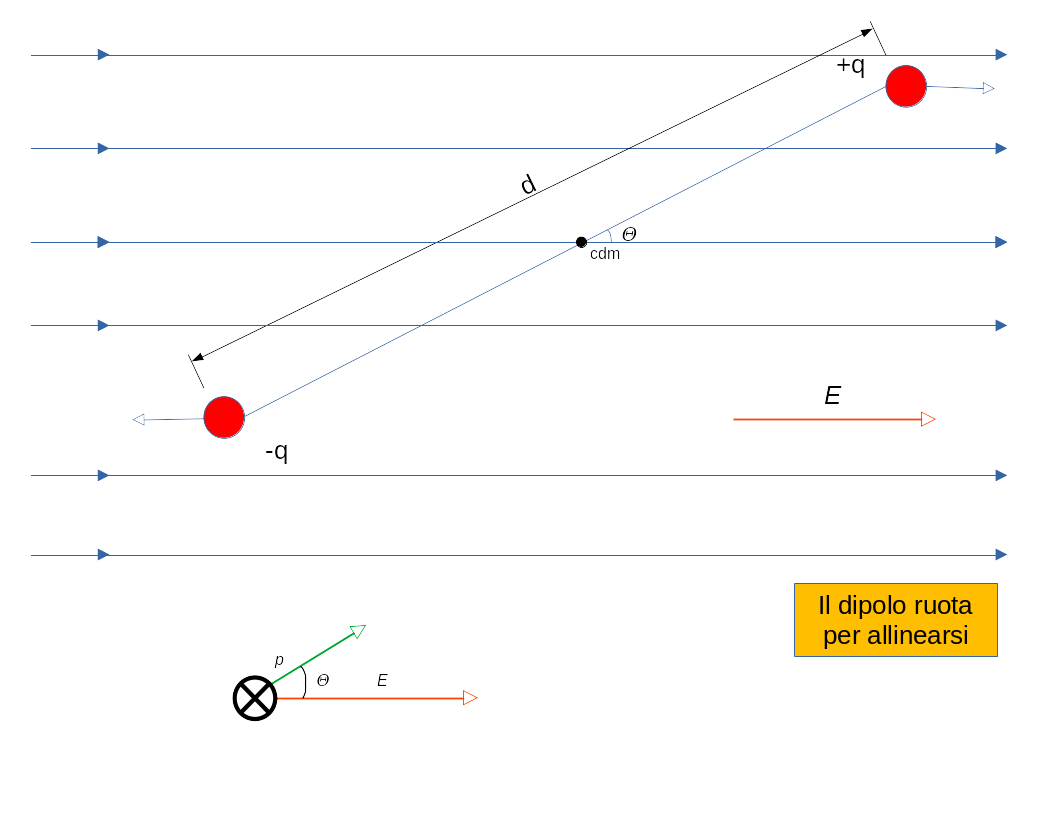
\includegraphics[height=8cm]{img/grafuci del dipolo elettrico.png}
\end{figure}
$\vec{F} (+q) e \vec{F} (-q)$ hanno intensità uguali e direzioni opposta. La forza netta è zero, ma esercitano un \textbf{momento torcente} $\vec{\uptau}$:
\begin{equation}
\uptau=-Fd \sin {\texttheta} = -pE sin {\texttheta}
\end{equation}
(\textit{segno meno perché il verso è orario}).
In forma vettore: $\vec{\uptau}=\vec{p}*\vec{E}$
\section{Energia potenziale di un dipolo elettrico}
L'energia potenziale $U$ di un dipolo elettrico $\vec{p}$ dipende dal suo \textit{orientamento}.
$U$ è minimo quando $\vec{p}$ è allineaTo Con il campo $\vec{E}$ - Nel mimimo è in equilibro:
$\abs{\vec{\uptau}}=\abs{p}\abs{E}\sin \texttheta=0$. Scegliamo $U=0$ per $\texttheta=90^o$.\\
L'energia potenziale diventa
\begin{equation}
  U=-L=\int^{\texttheta}_{90^o}\uptau d \texttheta= \int^{\texttheta}_{90^o} pE\sin \texttheta d\texttheta =-pE\cos\texttheta
\end{equation}
In forma vettoriale: $U=-\vec{p}*\vec{E}$
\section{Problema}
\begin{tasks}
  \task A quale distanza si trovano i cewntri delle cariche positiva e negativa di una molecola d'acqua?
  \begin{eqnarray*}
    p=qd\to d=\frac{p}{q}\\
    p(H_2O)=10e=1,6*10^{-30}C\\
    q(H_2O))10e)=1,6*10^{-18}C\\
    d=\frac{p}{q}=\frac{6,2*10^{-30}Cm}{1,6*10^{-18}C}=3,9*10^{-12}m=3,9pm
  \end{eqnarray*}
  \task Qual'è la differenza di energia potenziale tra le orientazioni $\texttheta=0^o$ e $\texttheta=180^o$ in un campo esterno $E=1,5*10^4\frac{N}{C}$?
  \begin{equation}
	\Delta U=2pE=2*6,2*10^{-30}Cm*1,5*10^3\frac{N}{C}=1,9*10^{-25}J
  \end{equation}
\end{tasks}

\chapter{La legge di Gauss}
\section{L'aspetto fisico}
Per calcolare il campo elettrico $\vec{E}$ di una distribuzione di carica si può \textbf{sommare} (integrare). La procedura è \textit{laboriosa}. Se esiste la simmetria, possiamo utilizzare un metodo più semplòice che sfrutta la relazione tra carica e campo, la \textbf{legge di Gauss}
\section{La superficie Gaussiana}
Scegliamo una superficie Gaussiana ({\it cioè una superficie chiusa}) intorno ad una carica.
Per la carica puntiforme, la {\bf sfera} è la superficie più simmetrica.
Le linee di campo intercettano la superficie.
\begin{tasks}
  \task Per una carica $Q$ il campo è $E=\frac{kQ}{r^2}$
  \task Per una carica 2Q, più linee intercettano la superficie
  \task la carica è $-\frac{Q}{2}$
\end{tasks}
Serve una grandezza che \textbf{quantifica} quanto una superificie è attraversata da un campo.
\section {Il flusso elettrico}
Un campo $\vec{E}$ attraversa un elemento di superficie $\Delta \vec{A}$ \texttt{vettore di area $\Delta \vec{A}$: \textbf{perpendicolare} alla superficie}.\\ Definizione del flusso elettrico $\Delta \vec{\upphi}$:
\begin{equation}
	\Delta \upphi =\vec{E}*\Delta\vec{A}=E\Delta A\cos\texttheta
\end{equation}
Per l'\textit{intera} superficie:
$\upphi = \sigma \vec{E}*\Delta \vec{A}=\int \vec{E}*d\vec{A}$ - Per una superficie chiusa, l'orientamento di $\Delta \vec{A}$ è uscente.
\begin{itemize}
\item $\vec{E}$ uscente contribuisce $\Delta \upphi >0$
\item $\vec{E}$ entrante contribuisce $\Delta \upphi <0$
\item $\vec{E} || \Delta \vec{A}$ da $\Delta \upphi =0$
\end{itemize}
Il flusso netto di una superficie chiusa è
\begin{equation}
	\upphi=\oint \vec{E}*d\vec{A}
\end{equation}
\section{Cilindro in campo uniforme}
Superficie guessiana a forma di \textbf{cilindro} di raggio \textit{R}. Campo elettrico $\vec{E}$
\textbf{uniforme}, parallelo all'asse. Quanto vale il fluso netto?
\begin{equation}
  \upphi=\oint \vec{E}*d\vec{A}=\int_a \vec{E}*d\vec{A}+\int_b\vec{E}*d\vec{A}+\int_c \vec{E}*
  d\vec{A}
\end{equation}
\begin{itemize}
\item $\int_a \vec{E}*d\vec{A}=-\pi R^2E$
\item $\int_b \vec{E}*d\vec{A}=0$
\item $\int_c\vec{E}*d\vec{A}=\pi R^2E$
\item $\upphi =0$  
\end{itemize}
\section{La legge di Gauss}
Relazione tra il flusso $\upphi$ attraverso una superficie chiusa e la carica netta $q_{int}$ racchiusa all'interno della superficie:
\begin{equation}
	\xi_0\upphi=q_{int} \text{ o } \xi_0\oint \vec{E}*d\vec{A}=q_{int}
\end{equation}
\begin{itemize}
\item \textit{se $q_{int}$ è positiva, il flusso netto è uscente}
\item \textit{se $q_{int}$ è negativo, il flusso netto è entrante}
\end{itemize}
Una carica esterna alla superficie può cambiare $\vec{E}$ localmente, ma non influisce sul flusso totale.
\begin{figure}[!h]
 	\centering
	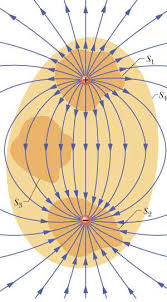
\includegraphics[height=5cm]{img/cariche opposte.jpg}
    	\caption{Due cariche di intensità uguale, ma di segno opposto}
\end{figure}
\begin{itemize}
\item $S_1$: $\vec{E}$ uscente in tutti i punti. $\Phi$ positivo, $q_{int}$ negativa
\item $S_2$: $\vec{E}$ entrante in tutti i punti. $\Phi$ negativa, $q_{int}$ negativa
\item $S_3$ Non racchiude nessuna carica. Ogni linea di campo che entra, esce, quindi $\Phi = 0$
  \item $S_4$ $q_{int}$ = $Q-Q=0$, quindi $\Phi = 0$
\end{itemize}

\section{La legge di Gauss e di Coulomb}
Racchiudiamo una \textbf{carica puntiforme} in una superficie sferica di raggio $r$.
Per simmetria, il campo elettronico ha il medesimo modulo $E$ su \textbf{tutti i punti della sfera}.\\
Applichiamo Gauss:
\begin{eqnarray*}
  \xi_0\oint \vec{E}*d\vec{A}=q_{int}\\
  \xi_0 E(4\pi r^2) = q\\
  E=\frac{q}{4\pi\xi_0r^2}
\end{eqnarray*}
Cioè, la legge di coulomb!
\subsection{Problema svolto}
Guscio sferica di raggio $R=10cm$ - dotato di carica uniforme $Q=-16e$ - Al centro carca puntiforme $q=5e$. Calcolare il campo $\vec{E}$
\begin{itemize}
\item nel punto $P_1$ a $r_1=6cm$
\item nel punto $P_2$ a $r_2=12cm$
\end{itemize}
\begin{eqnarray*}
  \xi_0 E_1(4\pi r_1^2)=q\to E=\frac{q}{4\pi \xi_0 r^2_1}=\frac{4e}{4\pi \xi_0 (0,06m)^2}=2,0*10^{-6}\frac{N}{C} \text{ verso l'esterno}\\
  \xi_0 E_2 (4\pi r^2_2)=q+Q\to \frac{q+Q}{4\pi \xi_0 r^2_2}=\frac{4e}{4\pi \xi_0 (0,12m)^2}=1,1 *10^{-6}\frac{N}{C} \text{ verso l'interno}
\end{eqnarray*}
\section{Un conduttore carico isolato}
Il campo elettrico all'\textit{interno} di un conduttore in equilibrio elettrostatico è \textit{nullo}
\begin{center}
	se no, si spostano le cariche
\end{center}
Scegliamo una superficie gaussiana appena sotto la superficie. $E=0\to \phi=0\to q_{int}=0$\\
L'eccesso di carica su un conduttore isolato si dispone totalmente sulla
\textbf{superficie esterna}. Anche una superficie gaussiana che racchiude \textbf{una cavita} ha
$E=0 \to \phi=0\to q_{int}=0$. La superficie di una cavità interna di un conduttore \textbf{non ha carica} in eccesso.\\
In generale, la carica \textit{non} si distribuisce uniformemente sulla superficie di un conduttore. Però c'è una relazione diretta tra il \textbf{campo} \textit{E} e la \textbf{densità di carica} $\sigma$. Considera un ciindro che racchiude un elemento di superficie - Il campo $E$ è
\textbf {perpendicolare} alla superficie
\begin{center}
	{\it se no si sposta la carica}
\end{center}
applicando Gauss: $\xi_0 \oint \vec{E}*d\vec{A}=q_{int}\to \xi_0EA=\sigma A \to E=\frac{\sigma}{\xi_0}$
\subsection{Problema svolto}
Una carica puntiforme di $Q=-5\mu C$ è posta all'interno di un guscio sferico metallico di raggio interno $R$, spostato di una distanza $\frac{R}{2}$ dal centro.
\begin{itemize}
\item Qual'è la carica indotta?
\item Qual'è l'andamento del campo interno ed esterno?
\end{itemize}
$Q$ induce un carica positiva $+5\mu C$ di all'interno, distribuita in modo \textbf{non-uniforme}.
Il campo all'interno è asimmetrico. La parete interna ha una carica di $-5\mu C$ distribuita in modo \textbf{uniforme}. Il campo esterno è simmetrico, come il campo di una carica puntiforme.
\section{Gauss per simmetria cilidrica}
Una bacchetta di plastica, di lunghezza infinita, densità di carica pari a $\lambda C/m$, Com'è il campo $\vec{E}$ a distanza $r$? Fruttare l'integrale è davvero faticoso\dots Applichiamo Gausss per la \textbf{superficie cilintrica} di altezza $h$. Per simmetria, $\vec{E}$ ha direzione \textbf{radiale}.
\begin{equation}
\xi_9\oint \vec{E}*d\vec{A}=q_{int}\to \xi_0 E2\pi hr=\lambda h\to E=\frac{\lambda}{2\pi r\xi_0}
\end{equation}
vake se la distanza dell'estremità è molto minore di $r$.
\section{Gauss per simmetria piana}
Una lamina isolante sottile, con una densità di carica superficiale $\sigma \frac{C}{m^2}$.
\paragraph{Superficie gaussiana:} cilindro di base $A$. Per simmetria, $\vec{E}$ perpendicolare alla lamina.\\ Applichiamo Guass: $\xi \oint \vec{E}*d\vec{A}=q_{int} \to \xi_0E2A=\sigma A\to E=\frac{\sigma}{2\xi_0}$\\
Concorda con il risultato trovato per il disco $E=\frac{\sigma}{2\xi_0}\left(1-\frac{z}{\sqrt{(R^2+z^2)}}\right)$\\
Per una piastra conduttrice la carica si distribuisce sulla superficie. Senza campo esterno, la carica è uguale da ambi lati, $\sigma_1=\sigma/2$. Identico, ma con verso di $E$ opposto, per carica negativa. Messe una a cando all'altra, le cariche sono attratte verso l'intrno. Il campo in mezzo diventa $E=\frac{2\sigma_1}{\xi_0}=\frac{\sigma}{\xi_0}$
\section{Gauss per simmetria sferica}
Con Gauss dimostriamo i 2 teoremi dei gusci. Guscio sferico di carica totale $q$ e raggio $R$.
\begin{enumerate}
\item \textit{Una superficie unifomemente carica attrae o respinge una carica esterna come se tutta la carica fosse concentrata nel suo centro.} Applicare Gauss alla superficie $S_2: E=\frac{q}{4\pi \xi_0 r^2}$ per $(r>R)$
  \item \textit{Una carica posta all'interno di una superficie chiusa uniformemente carica non ne sente la forza.} Applicare Gauss alla superficie $S_2: E=q_{int}=0$ per $(r<R)$
\end{enumerate}
Ogni distribuzione con simmetira sfrefica è una sovrapposizione di strati concentrici. Densità di carica $p$ varia soltanto con $r$
\begin{equation}
  E=\frac{q^\prime}{4\pi\xi_0r^2}
\end{equation}
Per $p$ uniforme e $r<R$
\begin{equation}
  	\frac{q^\prime}{\frac{4}{3}\pi r^3}=\frac{q}{\frac{4}{3}\pi R^3}\to q^\prime=q\frac{r^3}{R^3}
\end{equation}
per ci $E=\frac{qr}{4\pi \xi_0 R^3}$

\chapter{Potenziale elettrico}
\section{L'aspetto fisico}
La forza elettrostatica è \textbf{conservativa}, per cui, si può associarvi un'\textbf{energia potenziale}. La \textbf{conservazione} dell'energia meccanica semplifica molti calcoli. $q_2$ senta la \textbf{forza} $\vec{F}$ di $q_1$. Alla posizione di $q_2$ c'è un \textbf{campo} $\vec{E}=\vec{F}/q_2$ - $q_2$ ha un \textbf{energia potenziale} \textit{U} dovuta a $q_1$. Alla posizione di $q_2$ c'è un \textbf{potenziale elettrico} $V=\frac{U}{q_2}$ (\textbf{Nota bene:} grandezza scalare!)
\section{Il potenziale elettrico}
L'energia potenziale \textit{U}: $U=0$ a un \textbf{livello di riferimento}. Spostando, la forza conservativa compie un \textbf{lavoro} $L$. L'energia potenziale è $E=-L$. Scegliamo $U=0$ a \textbf{carica esplorativa} $q_0$ viene trasportata da $\infty$ a $P$.\\
$L_\infty$ è il lavoro svolto \textbf{dalla forza elettrica} per il trasporto. Il potenziale elettrico nel punto $P$: $V=\frac{-L_\infty}{q_0}$. Ad ogni posizione interno ad una carica è assegnato un potenziale elettrico.
\section{Unità di misura}
Il potenziale elettrico viene espresso in $\frac{J}{C}$ o V (\textbf{Volt}).\\
Figura anche in altre unità:
\begin{center}
  Il campo elettrico $1\frac{N}{C}=1\frac{V}{m}$
\end{center}
L'energia per il \textbf{sistema microscopici}: $1eV=1,6*10^{-19}$
\begin{center}
  \textit{\color{blue} $1eV$ è la differenza in energia di un elettrone che attraverso una differenza di potenziale di 1V}
\end{center}
\section{Il potenziale elettrico}
\paragraph{Inversamente:} una carica $q$ in un potenziale elettrico $V$ ha energia potenziale $U=qV$. Spostanedosi in un compo elettrico da $i$ e $f$ abbiamo differenza di potenziale $\Delta V=V_f-V_i$. Per una carica $q: \Delta U=q\Delta V=q(V_f-V_i)=-L$, $\Delta V \text{ } \Delta U$ \textbf{non dipendono dal cammino} da $i$ a $f$.\\
Possibile applicare la \textbf{conservazione dell'energia meccanica: } $U_i+K_i=U_f+K_f$ per cui $\Delta K=K_f-K_i=-q\Delta V$ - Se agisce sulla particella anche un'altra forza che compie un lavoro $L_{app}$, abbiamo $\Delta K=-q\Delta V+L_{L_{app}}$.
\section{Superfici equipotenziali}
L'insieme dei punti con lo \textbf{stezzo potenziale} forma una superficie: La superficie equipotenziale. Spostando una carica tra due punti di una superficie equipotenziale, il campo elettrico \textbf{non compie lavoro}.\\
Spostamenti \textbf{sulla} superficie hanno $L=0$, per cui $L=\vec{F}*\vec{d}=q \text{ } \vec{E}*\vec{d}=qEd\cos\theta=0\to \theta =90^o$\\
La superficie equipotenziale è perpendicolare a $\vec{E}$
\begin{itemize}
\item \textit{Per un campo uniforme: piani perpendicolari a $\vec{E}$}
\item \textit{Per un carica puntiforme: sfere concentriche}
\end{itemize}
\section {Calcolo del potenziale, dato $\vec{E}$}
La Carica di prova $q_0$ si muove da $i$ e $f$. Lavoro svolto da $\vec{E}$ per spostamento $d\vec{s}$:
\begin{equation}
	dL=\vec{F}*d\vec{s}=q_0\vec{E}*d\vec{s}
\end{equation}
Per cui $V_f-V_i=-\frac{L}{q_0}=-\int^f_i \vec{E}*d\vec{s}$
\begin{center}
	Non dipende dal percorso?
\end{center}
Per campo uniforme:
\begin{equation}
  \Delta V=-\int_i^f \vec{E}*d\vec{s}=-E\Delta x
\end{equation}
\section{Potenziale di una carica puntiforma}
Potenziale $V$ per punto $P$ a distanza $R$ da carica $q$. $V=0$ a distanza infinita. $V_f-V_i=-\int^f_i\vec{E}*d\vec{s}$.\\
Libertà di scelta per il cammino. Lungo la direzione radiale: $\vec{E}*d\vec{s}=Edr0-V=-\int^\infty_REdr=-\int^\infty_R\frac{q}{4\pi \xi_0r}dr=-\frac{q}{4\pi \xi_0}\left[\frac{-1}{r}\right]^\infty_R=-\frac{q}{4\pi \xi_0 r}$\\
per cui $V=\frac{q}{4\pi\xi_or}$
\begin{itemize}
\item Carica positiva $\leftrightarrow$ potenziale positivo
\item Carica negativa $\leftrightarrow$ potenziale negativo
\end{itemize}
Valido anceh per distribuzione sferiche non-puntiforme
\section{Insieme di cariche puntiformi}
Il \textit{principio di sovrapposizione} vale anche per $V$, Per $n$ cariche, il potenziale netto sarà
\begin{equation}
  V=\sum_{i=1}^{n}V_i=\frac{1}{4\pi \xi_0}\sum_{i=1}^{n}\frac{q_i}{r_i}
\end{equation}
$Nb$: somma scalare!
\subsection{problema}
due protoni. Ordinare secondo i valori crescenti di $V$ nel punto $P$
\begin{equation}
  \begin{matrix}
    q_1=+12nC\\
    q_2=-24nC\\
    q_3=+31nC\\
    q_4=+17nC\\
    d=1,3m
  \end{matrix}
\end{equation}
Qual'è il potenziale nel punto P?
\begin{equation}
  V=\frac{1}{4\pi \xi_0}\sum_{i=1}^{n}\frac{q_i}{r_i}=
  \frac{1}{4\pi\xi_0}\left(\frac{q_1}{r_1}+\frac{q_2}{r_2}+\frac{q_3}{r_3}
    +\frac{q_4}{r_4}\right)=\frac{1}{4\pi\xi_0}
  \frac{(12-24+31+17)*10^{-9}}{\frac{1,3}{\sqrt{2}}}=352V
\end{equation}
\section{Potenziale di un dipolo elettrico}
Il potenziale in un in un punto arbitrario $P$ a distanza $r$, angolo $\Theta$:
\begin{equation}
  V=V_++V_- =\frac{1}{4\pi\xi_0}\left(\frac{q}{r_+} - \frac{q}{r_-}\right)=
  \frac{q}{4\pi\xi_0}\frac{r_--r_+}{r_+r_-}
\end{equation}
Per $r>>d:r_--r_+\approx d \cos\Theta,\text{ } r_+r_-\approx r^2$
\begin{equation*}
  \to V = \frac{q}{4\pi\xi_0}\frac{d\cos \Theta}{r^2}=\frac{p\cos\Theta}{4\pi\xi_0}=
  \frac{\overrightarrow{p}*\hat{r}}{4\pi\xi_0}
\end{equation*}
Ove $\overrightarrow{r}$ è il momento dipolare -- \textit{\color{blue}il verso va da -q a +q}
\section{Potenziale di una distribuzione contitua}
Per distribuzione continua dividiamo in infinitesimi $dq$. Ogni infinitesimo $dq$ contribuisce $dV=\frac{dq}{4\pi\xi_0r}$, così $v=\frac{1}{4\pi\xi_0}\sum^n\limits_{i=0}\frac{q_i}{r_i}$ diventa $V=\frac{1}{4\pi\xi_0}\int \frac{dq}{r}$